\chapter{Design and Architecture}


\section{Overall Architecture}
One of the customer requirements was that a Content Provider be developed to provide access to the model for movement to be designed. Content providers function as data repositories that enable other applications to interact with the stored data. More specifically, content providers provide CRUD (create, retrieve, update, delete) functions. Content providers are intended to be used with a repository architecture. In a repository architecture, there is a central data repository which maintains the shared data between the components. The components only communicate directly with the repository, and are therefore independent of each other. This independence makes it easy to add or remove components from the application system, which was emphasized as a major requirement from the customer. While it is possible to embed a content provider within a single application, this causes the independence to be lost, nullifying the advantage of using a content provider in the first place.

The system that has been designed according to the repository architecture, and consists of five component apps, each of these components fulfills a well-defined role in the application system architecture:
\begin{description}
\item[Valens Content Provider] has the role of the repository in the repository architecture.
\item[Valens Health Helper] the proof-of-concept application. Demonstrates one simple way in which the data provided by the content provider can be used as a part of a health-promoting app.
\item[Valens Step Detector] the sensor model. The sensor model listens to the sensor data, and feeds the content provider with the timestamps of any detected steps.
\item[Valens Content Feeder] a service of deriving secondary data from the raw data provided by the step detector(s). This includes filtering out steps that have been counted by multiple step detectors to ensure that every step is counted just once, as well as deriving gait parameters. The code is integrated with the Content Providers APK for reasons of maintainability, but they are still logically independent.
\end{description}

\begin{figure}[p]

\setlength\fboxsep{0pt}
\setlength\fboxrule{1pt}\noindent\makebox[\textwidth]{%
 \fbox{
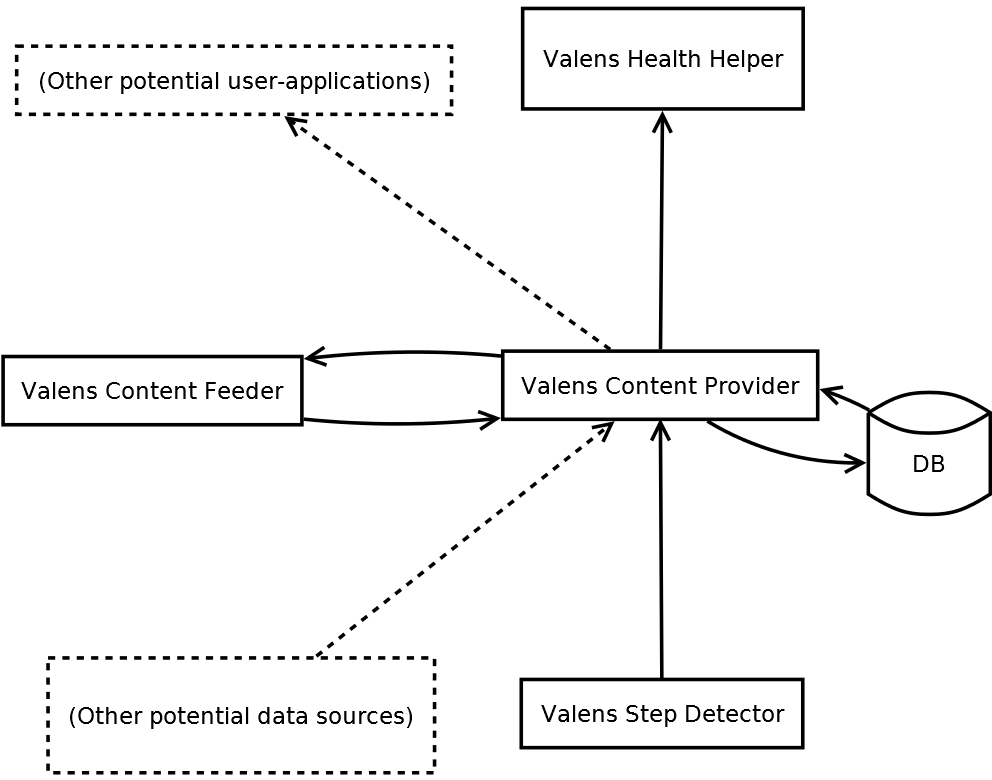
\includegraphics[width=1.45\textwidth , angle=0]{Res/OverallArchitecture}
}
}

\caption{The over-all system architecture}
\label{fig:Architecture}
\end{figure}


\section{Architecture of Valens Health Helper}
The application follows standard android application architecture, which is based on a Model-View-Controller (MVC) architecture. In a MVC architecture, which is a fairly common architecture for GUI-based applications, there are three components:

\begin{description}
\item[The model] contains the data and logic of the system.
\item[The view] is a visual representation of the data. 
\item[The controller] receives input and converts it into commands for the model or view. 
\end{description}

In Android, the view is described using XML layout files, the controller is defined using activity classes and the model is defined using the remaining Java classes. In practice, however, the android architecture does not separate the MVC components clearly. For instance, certain graphical features have to be implemented using the activity classes. Also, not a lot of effort was put into maintaining a pure MVC architecture.%TODO: Skal vi skrive dette?

Furthermore, in Android, an additional view layer separates the actual string values and other resources from the layout definitions. Resources are placed in a separate folder and files. The separation of layout and strings enables different localizations, so that the application can provide a user interface in different languages easily. 

In the android architecture, classes that inherit from the class Activity define a separate screen in the GUI. Because of this, a significant part of all the classes in the application are activity classes. These classes simply define the behaviour of their GUI screen. The flow for the GUI can be seen in Figure \ref{fig:GUIFlowchart}.



\begin{figure}
\setlength\fboxsep{0pt}
\setlength\fboxrule{1pt}\noindent\makebox[\textwidth]{
\fbox{
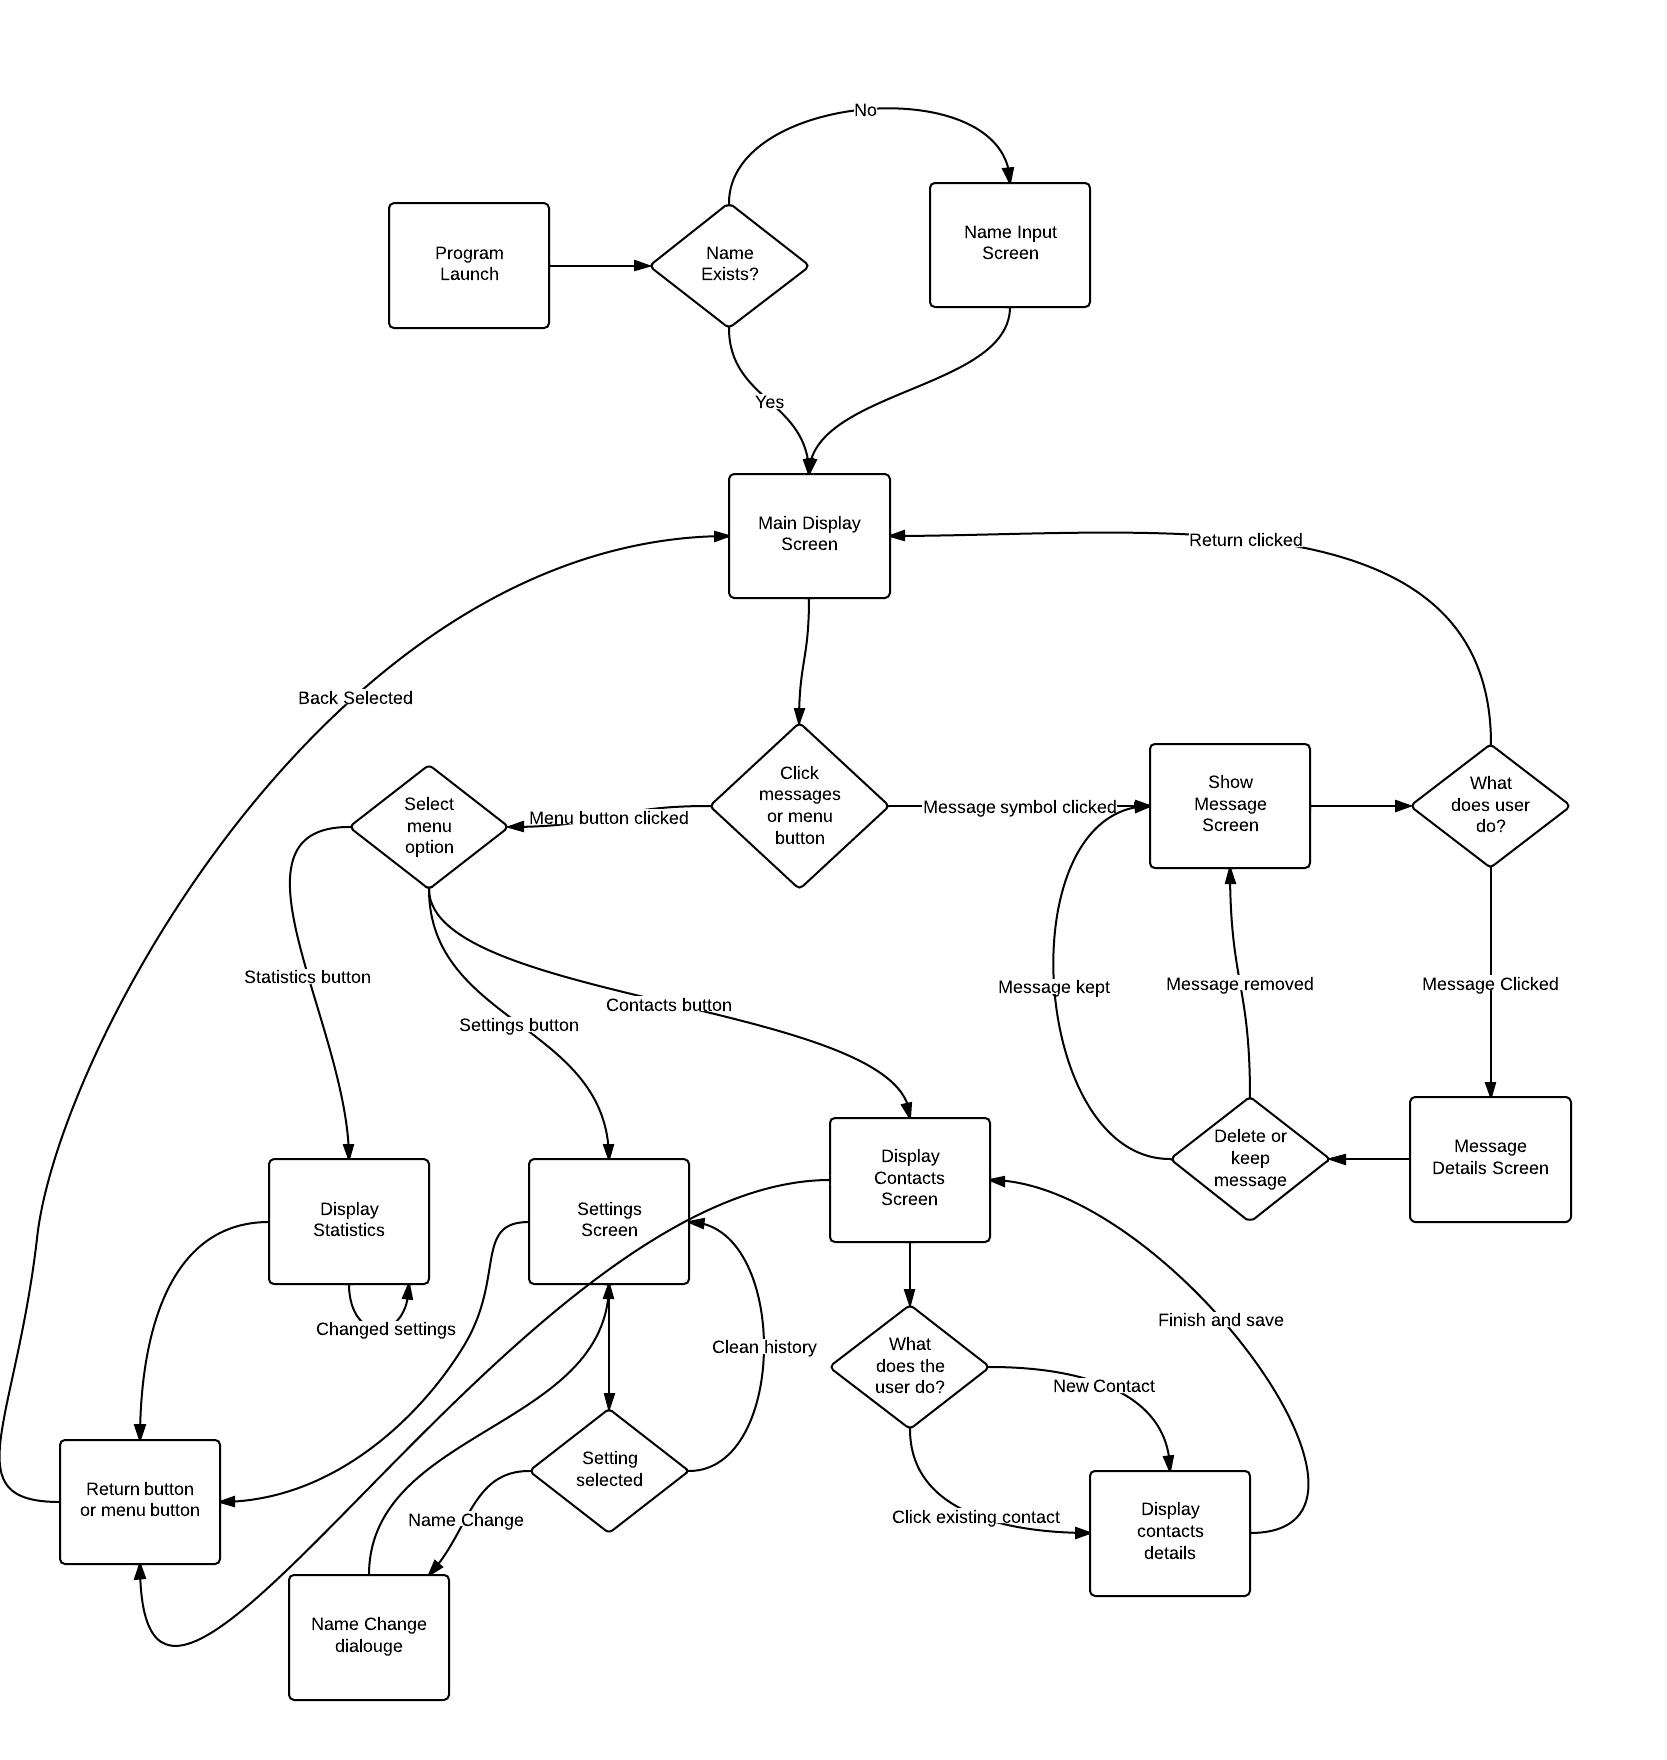
\includegraphics[width=1.2\textwidth, angle = 0]{Res/GUIFlowchart.png}
}
}
\caption{Flow chart describing the Graphical User Interface, grey lines mark features not used in the current application}
\label{fig:GUIFlowchart}
\end{figure}

\pagebreak


The definition of Activity classes are as following:
\begin{description}

\item[Activity classes]
define the activities employed in running the app. In Android, an \emph{Activity} is ``a single, focused thing that the user can do. Almost all activities interact with the user, so the Activity class takes care of creating a window for you in which you can place your UI"\footnote{http://developer.android.com/reference/android/app/Activity.html}. Every GUI screen corresponds to an activity, but not all activities need to have a GUI. In the current implementation, every activity except for \textit{LaunchActivity} has a GUI screen, so see the GUI flowchart for an overview of the activities used in the current implementation. 

\end{description}

Classes that are not activities can be roughly divided into four types: 

\begin{description}
\item[Connectivity classes]
provide an interface for communication with the database and content providers. There are three connectivity classes:
\begin{description}
\item[ContentProviderHelper] handles communication with the content provider. In particular, it contains several methods that sends queries to the Content Provider, interprets the data, and returns useful values to the GUI activities.
\item[DatabaseHelper] handles communication with the database. The database contains information necessary for the demo application to function, in particular events, messages and contact information.
\item[DatabaseContract] defines the strings used for table and column names in the database. While a DatabaseContract might seem redundant, it is common android application practice to use one. A database contract functions as a "contract" that define the legal interaction between the database and the application, by stating the legal table and column names.
\end{description}

\item[Data structure classes]
each define a useful data structure in the program. The data structure classes in the app are Contact, Event and RiskStatus.

\item[List adapter classes]
define how elements in a list should be displayed, and what kind of data should be associated with each element.
\newpage
\item[Widget classes]
define the functionality of the widget. There are two widget classes:
\begin{description}
\item[WidgetProvider] creates the widget and provides it with a GUI. Is called by the Android OS when the user creates the widget.
\item[WidgetUpdateService] takes care of updating the widget a regular intervals, by looking for new information in the content provider. Handles regular check with the help of an internal TimerTask class, Updater.
\end{description}
\end{description}
\section{Architecture of the Content Provider}
In android, Content Providers provide an interface to structured data of some sort. Access to for instance the list of contacts in the phone, or the phone's calendar is managed through standard content providers. Content Providers provide methods for inserting, updating and deleting relevant data. A major part of the assignment was to implement a Content Provider that gives developers access to structured movement data.

The Content Provider component is conceptually very simple, and consists of four classes:
\begin{description}
\item[CPValensDB]
a subclass of SQLiteOpenHelper, the standard android class for handling database communication. Specifies the procedure for creating the database, as well as upgrading and downgrading the database version. In the current implementation, upgrading and downgrading the database version clears all the data and tables, and creates the database according the details specified in the new database version. In the current version, creating the database consists of creating the tables given in the data model, without feeding any data into the database.
\item[DBSchema]
defines the database model and provides string values for the names of the tables and fields. Employing a database schema to demonstrate the structure of the database is standard in android applications.
\item[ValensDataProvider]
a subclass of ContentProvider, which is the standard android class for implementing content providers. This is the core of the content provider, and describes how queries to the content provider are handled.
\item[Main]
provdides the content provider with a basic GUI.
\end{description}

\section{Data model}

\section{Architecture of the Valens Step Detector}

Despite being a relatively simple application in terms of lines of code and GUI screens, the architecture of Valens Step Detector has a certain complexity.

\begin{description}

\item[LaunchActivity]
handles the basic GUI for the main screen.

\item[Values]
holds the values of the constants used for step detection.

\item[Methods]
contains most of the functions used for calculation of peaks.

\item[StepMainService]
is main class for the sensor model. Is implemented as an Android Service, and as such, it runs in the continually in the background until the user explicitly stops it. Functions as a SensorListener that listens to input from the accelerometer, and keeps track of the sensor vector lengths along with their timestamp. When enough data has been generated\footnote{Enough data is defined as $m+2k+2n$, where k is the size of the smoothing window, n is the size of the peak strength window, and m is a constant which defines how many time steps one wants to use for step detection. As the first and last $k+n$ steps are not used for step detection (see explanation of the algorithm in chapter \ref{def:coreAlgorithm}), only $m$ values will actually be used for step detection.} the StepMainService will launch a DetectStepsThread to detect steps in the given data, before clearing its data\footnote{For reasons that will be explained in the description of the algorithm, $2k+2n$ data points are retained.} to ensure that the maximum memory required by the service remains constant. 

\item[DetectStepsThread]
searches asynchronously for steps in the data provided to it. Step detection is performed in a separate thread so that sensor input is not interrupted by the calculation.

\item[Calibration Classes]
are a group of classes that are used for calibration, that is adjusting the mean and standard deviation to the step patterns of the user. There is one GUI class, one class used for timing and and one sensor class:
\begin{description}
\item[CalibrationActivity]
handles the GUI functions for the calibration screen. When the ``calibrate"-button is pressed, it starts a timer that starts the CalibrationStartTask after a certain amount of time has passed, so that the user has time to lock the screen and put the phone in his/her pocket.
\item[CalibrationStartTask]
is a TimerTask that simply plays a sound to indicate that calibration commences, and immediately starts an CalibrationThread. This class only exists because Java requires a TimerTask for the Timer to work properly, and CalibrationActivity can't inherit from TimerTask as it already inherits from Activity and Java does not support multiple inheritance. 
\item[CalibrationThread]
handles sensor input during calibration. When the calibration time has ended, it stops receiving input, calculates $\mu$ and $\sigma$, and terminates.
\end{description}
 
\end{description}
\section{Class description and diagram}

The class structures of the applications are relatively complex, as can be seen from the class diagrams in figures \ref{fig:DemoClassDiagram}, \ref{fig:CPClassDiagram} and \ref{fig:StepDetectClassDiagram}. As the class diagrams can be hard to read in the paper format, it is recommended to read the digital version on the application website\footnote{\url{http://valens.brennhe.it/\#documentation}}. The class diagrams are not the recommended way to understand the structure of the code, it would be better to consult the textual description above as well as the JavaDocs\footnote{\url{http://valens.brennhe.it/javadoc/}}.

\begin{figure}[p]

\caption{Class diagram for the demo application}
\label{fig:DemoClassDiagram}

\setlength\fboxsep{0pt}
\setlength\fboxrule{1pt}
\fbox{
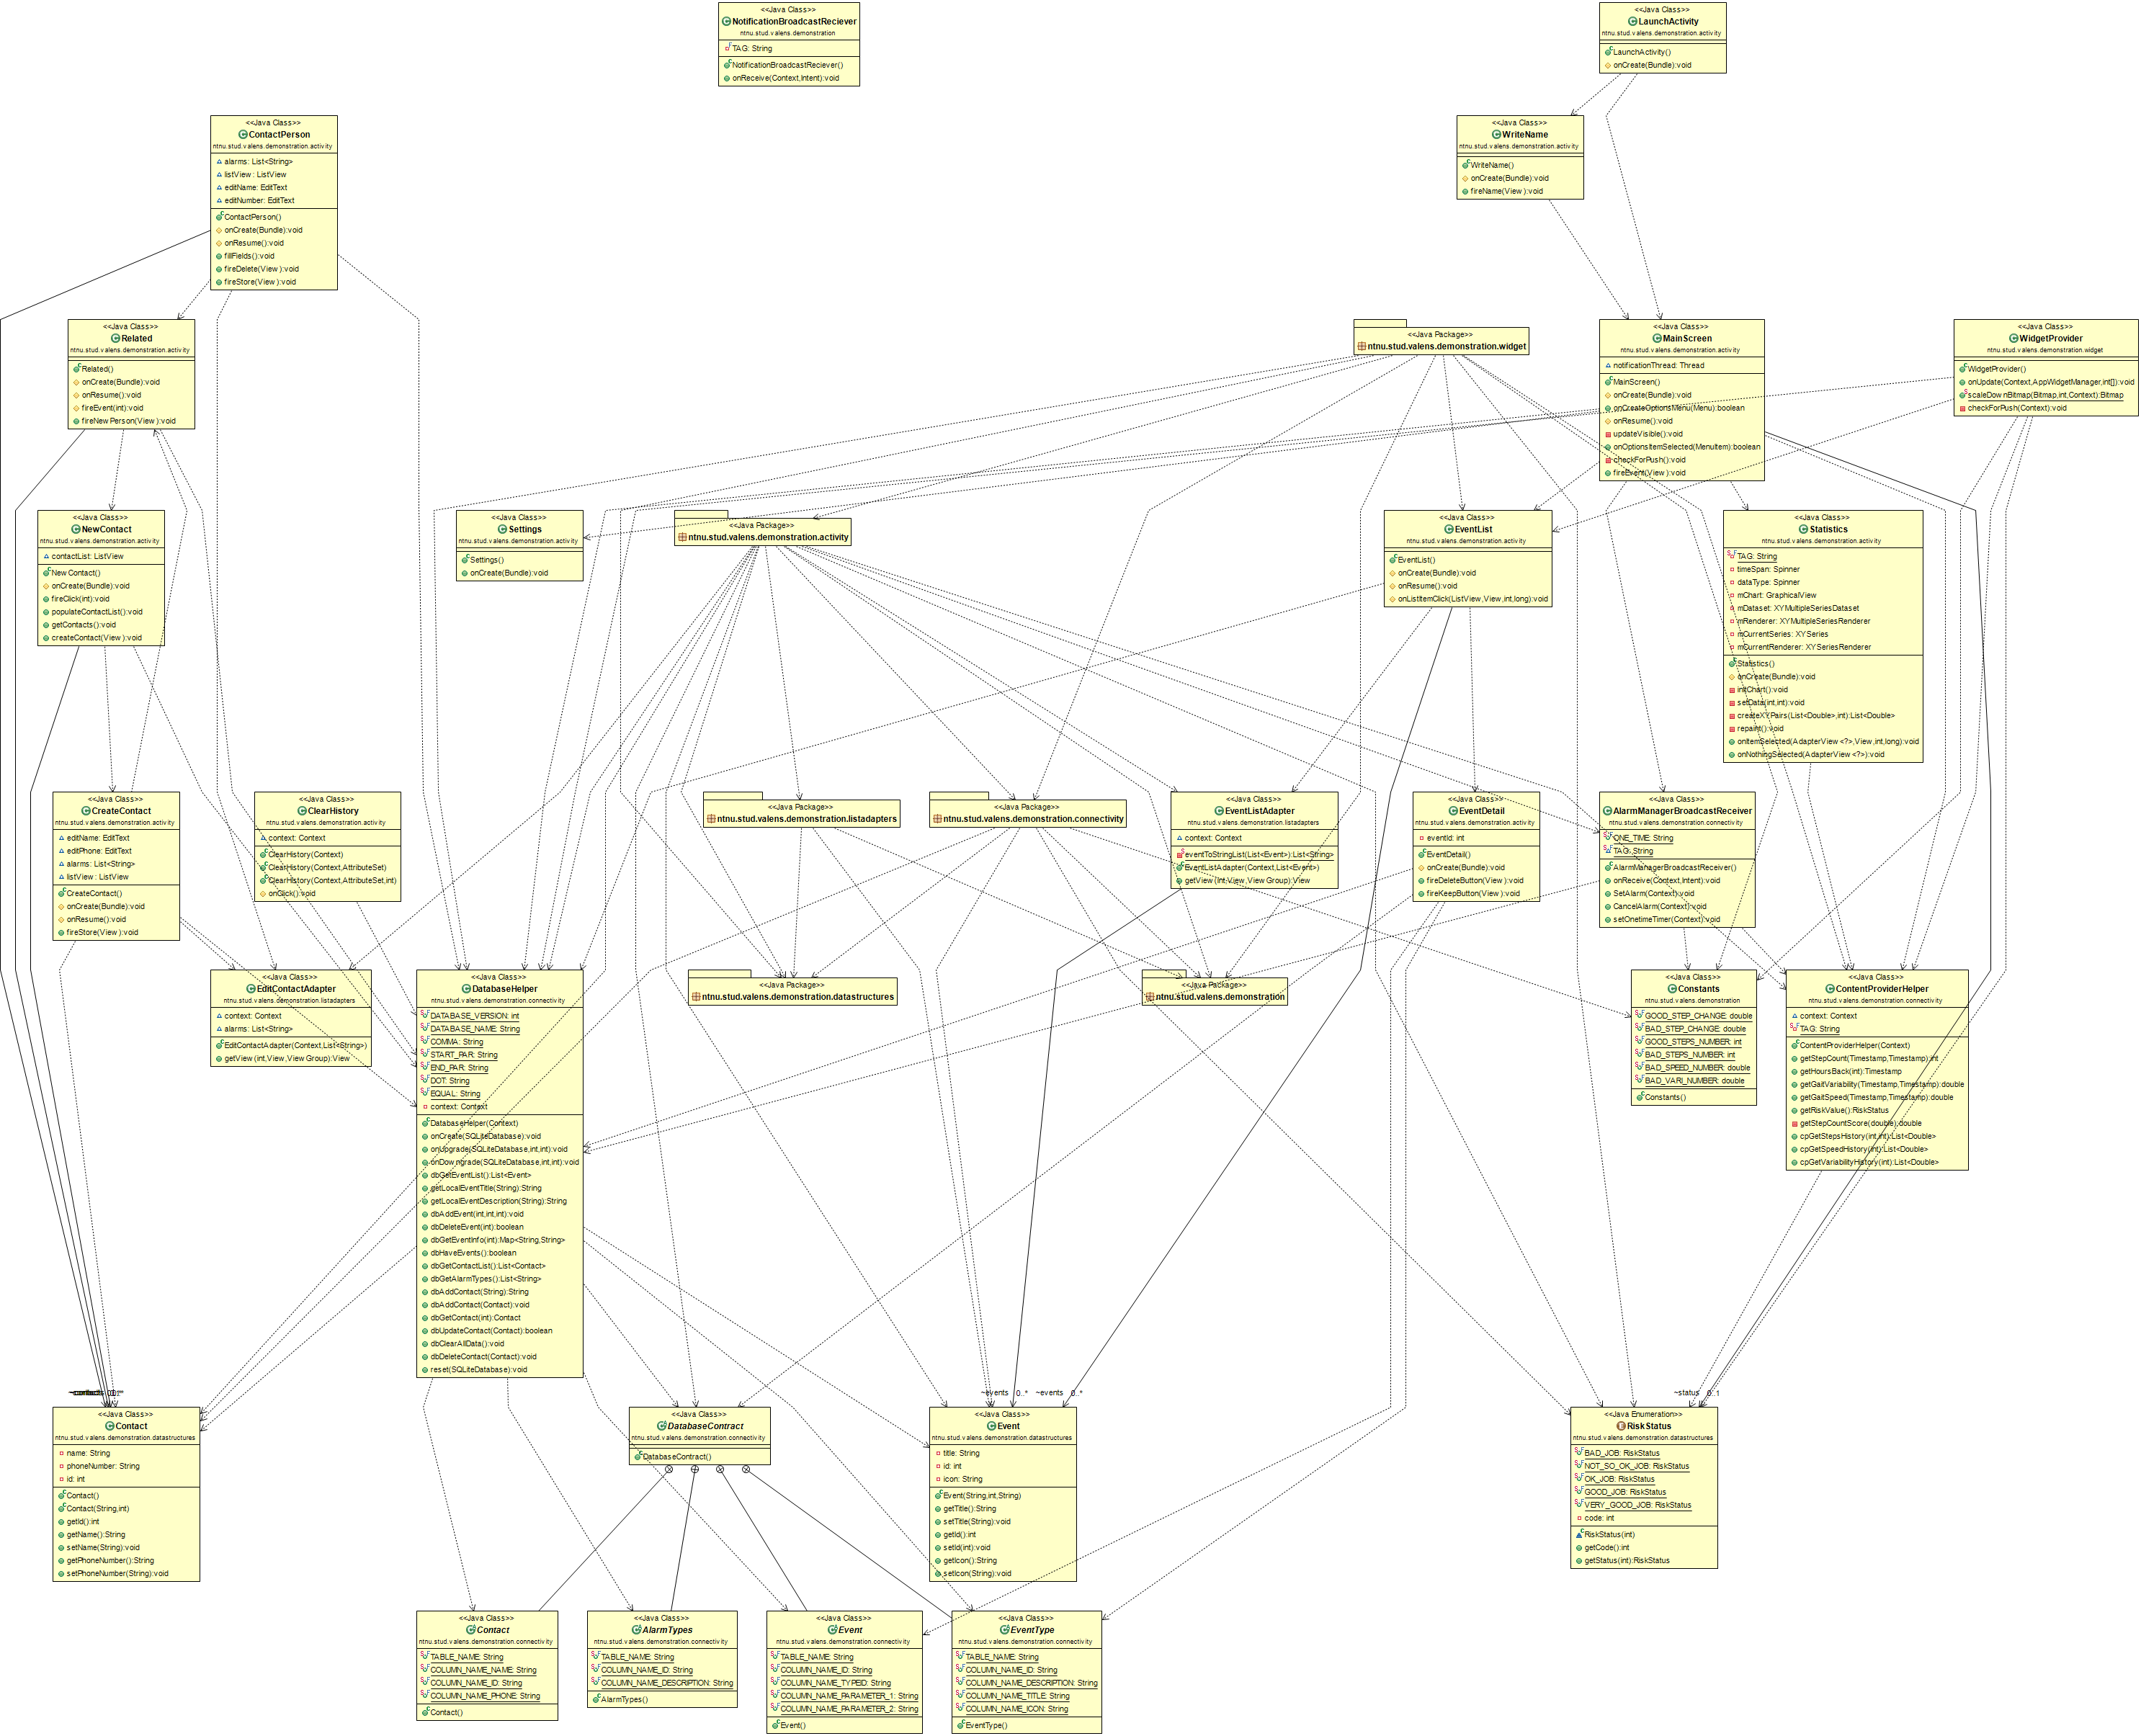
\includegraphics[width=1.2\textwidth, angle = 270]{Res/ClassDiagramDemonstration}
}

\end{figure}

\begin{figure}[p]

\caption{Class diagram of the content provider application}
\label{fig:CPClassDiagrarm}

\setlength\fboxsep{0pt}
\setlength\fboxrule{1pt}
\fbox{
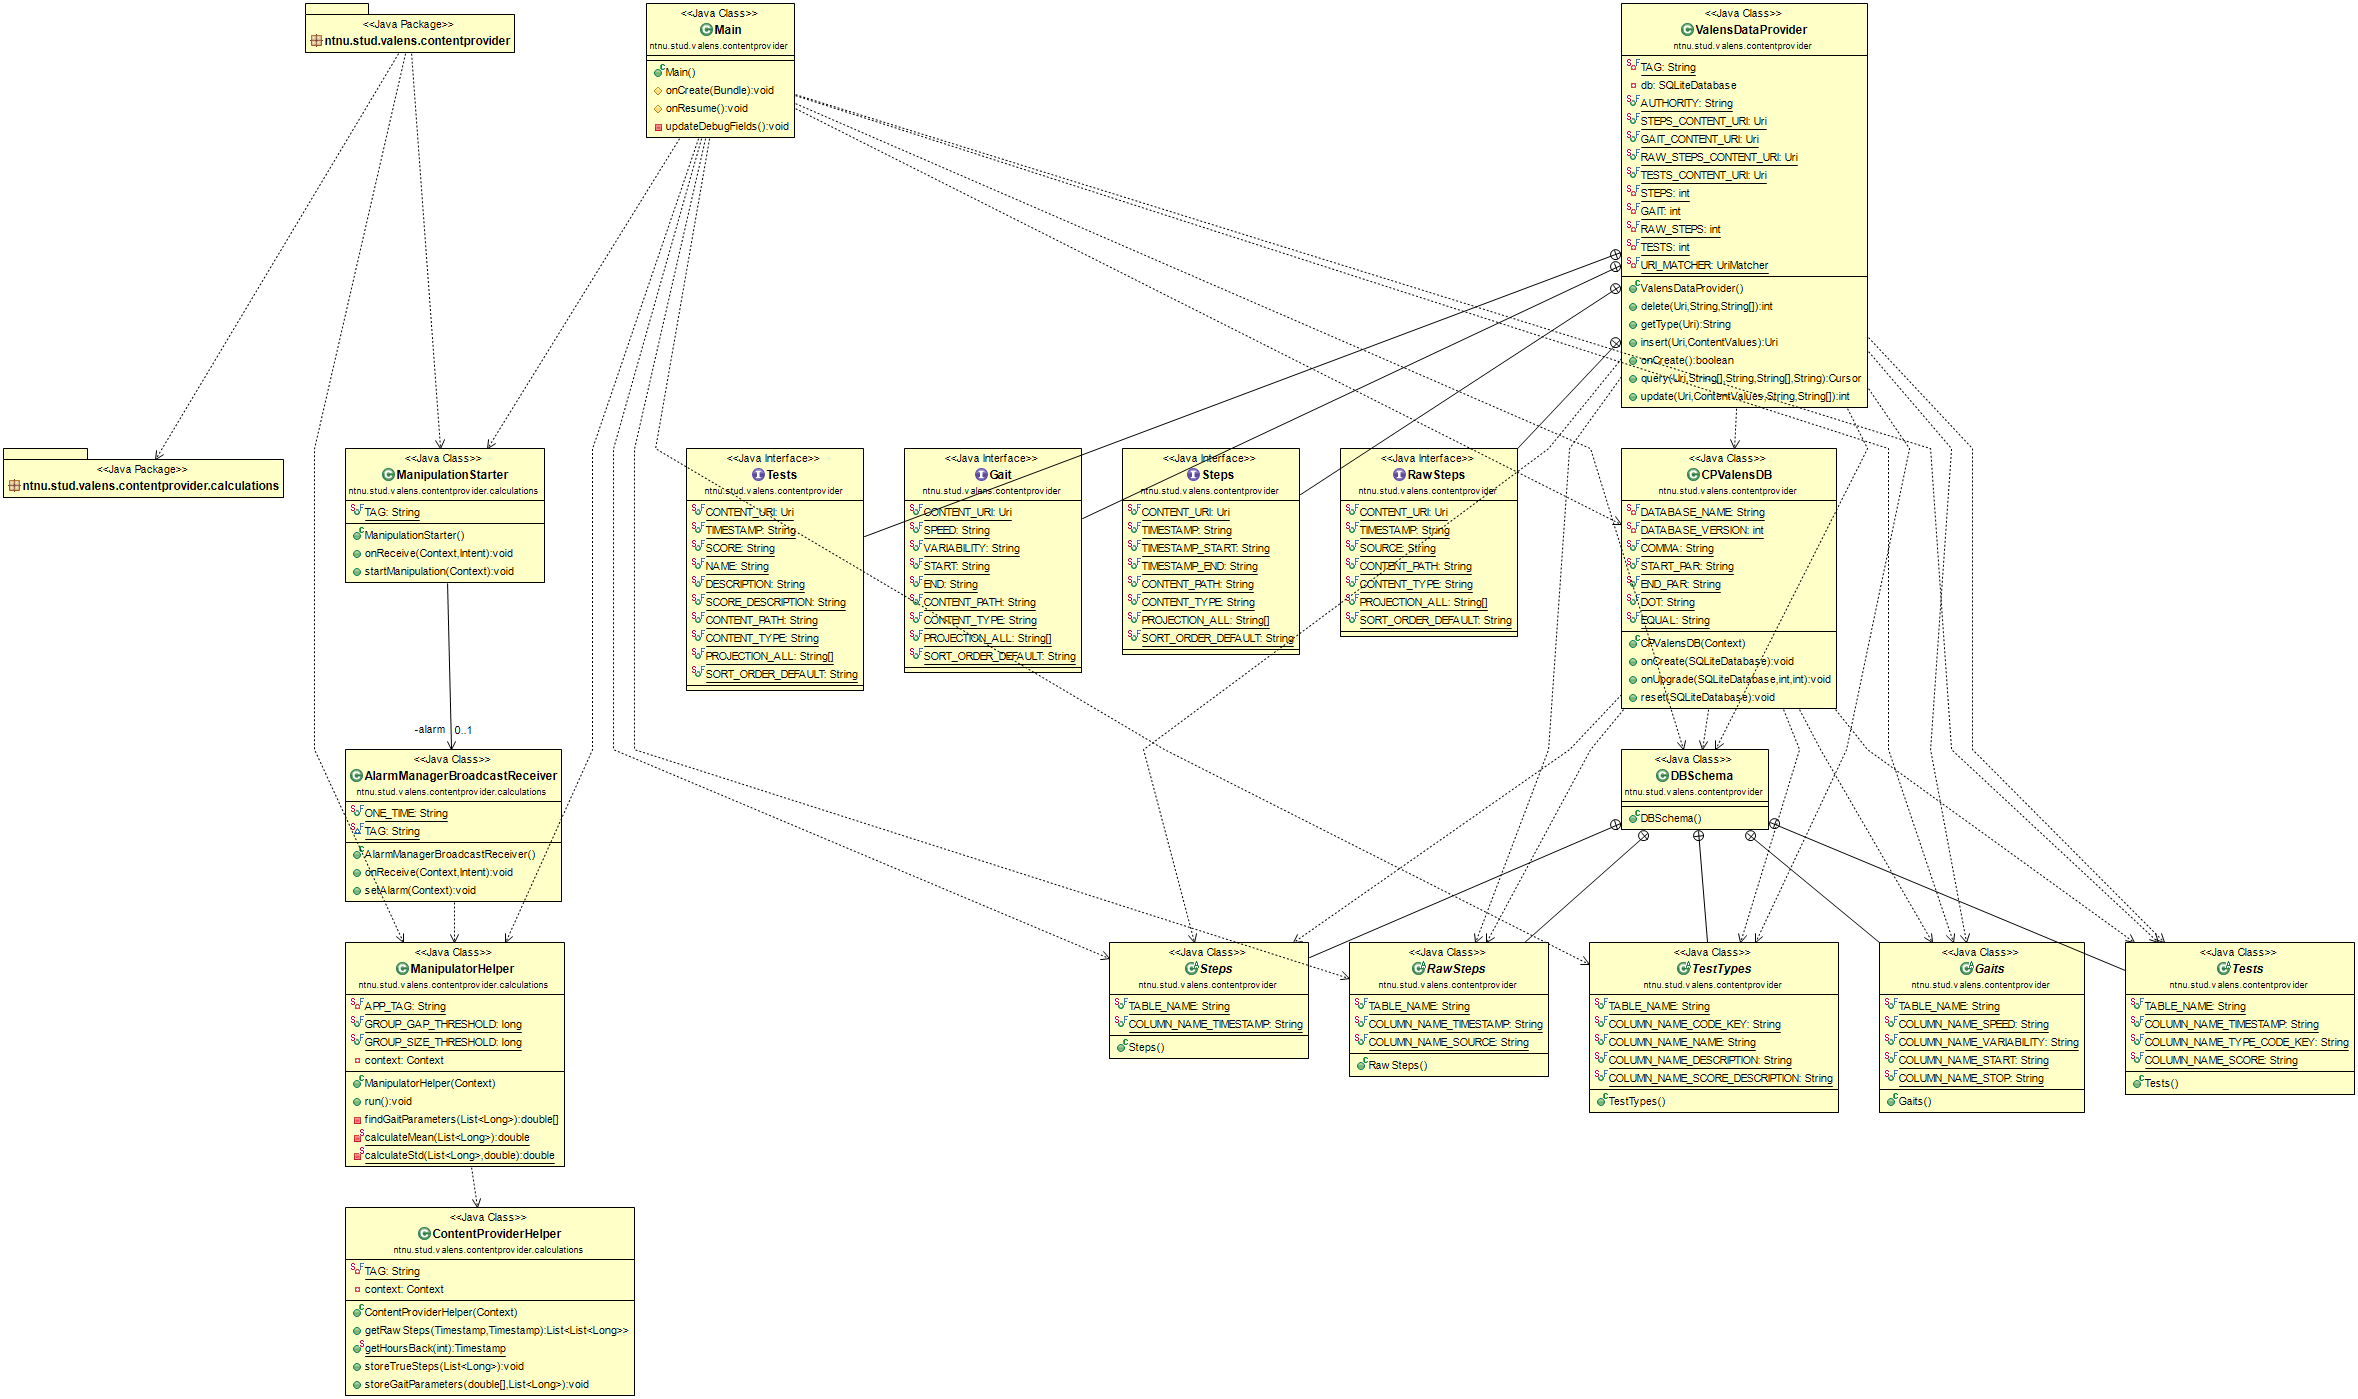
\includegraphics[width=1.2\textwidth, angle = 270]{Res/ClassDiagramContentProvider}
}

\end{figure}



\begin{figure}[p]

\caption{Class diagram for the step detector application}
\label{fig:StepDetectClassDiagram}

\setlength\fboxsep{0pt}
\setlength\fboxrule{1pt}
\fbox{
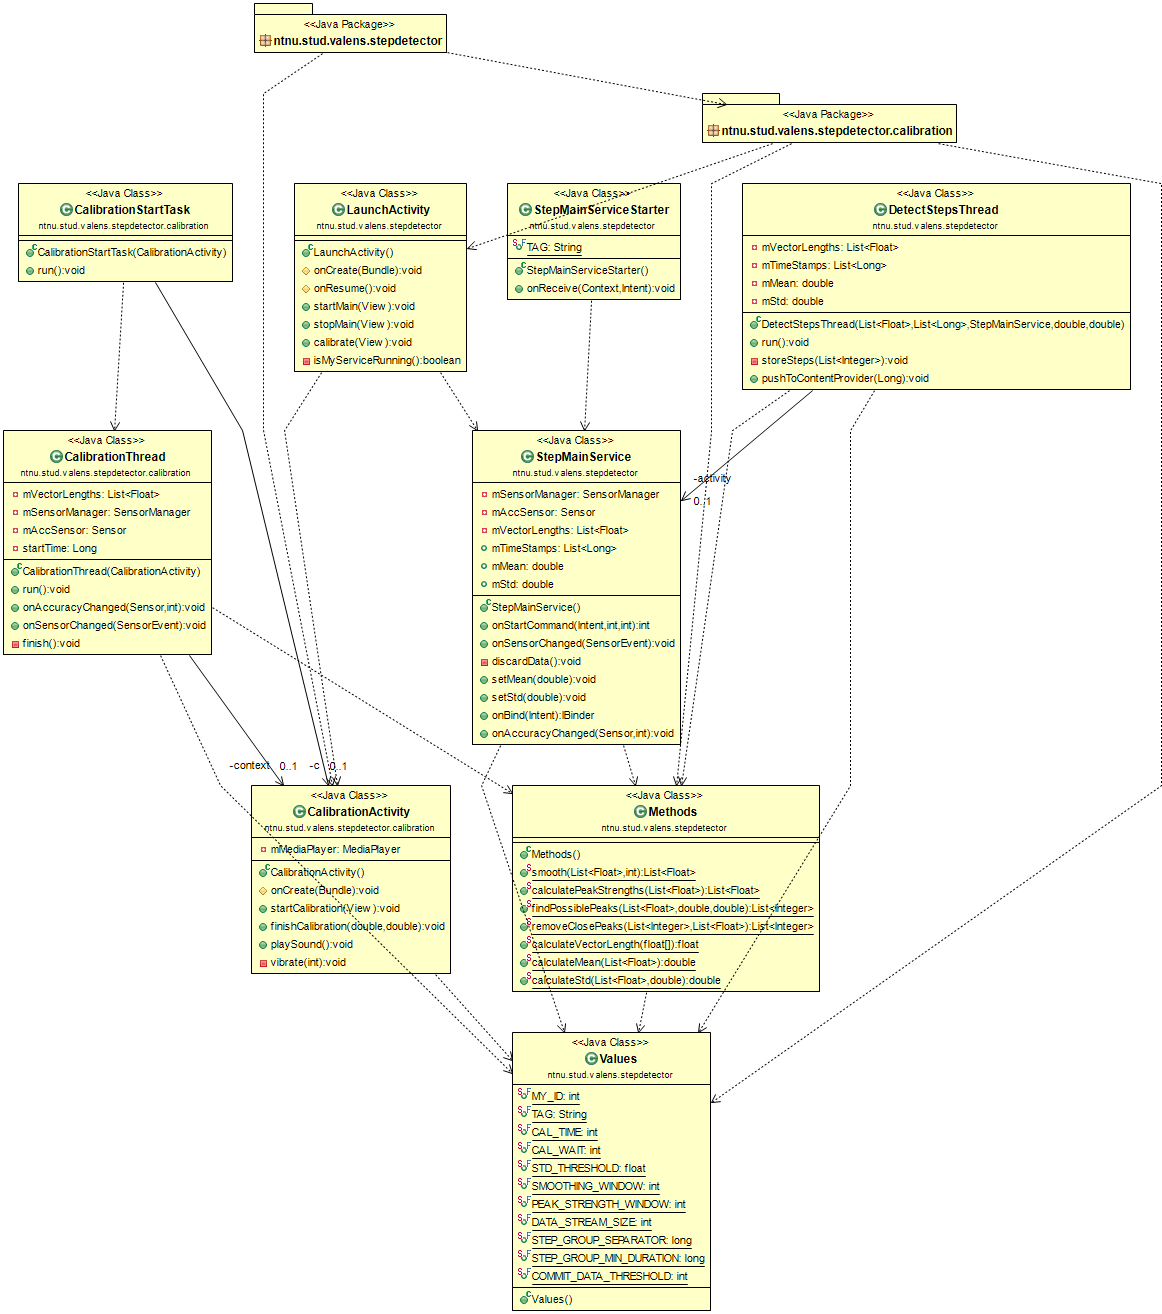
\includegraphics[width=1\textwidth, angle = 270]{Res/ClassDiagramStepDetector}
}

\end{figure}
\input{translation}


